\chapter{Introducción}

Los terremotos representan uno de los fenómenos naturales más devastadores, con un impacto significativo en la vida humana, las infraestructuras y las economías globales. Un terremoto se produce debido al movimiento súbito de las placas tectónicas de la Tierra, liberando una enorme cantidad de energía en forma de ondas sísmicas. Estas ondas pueden causar una destrucción masiva y pérdidas humanas, por lo que la detección temprana y precisa de terremotos es de vital importancia para mitigar sus efectos destructivos \cite{Joswig} \cite{havskov2008processing}.

Las ondas sísmicas generadas por un terremoto se dividen principalmente en dos tipos: las ondas P (primarias) y las ondas S (secundarias). Las ondas P son las primeras en llegar a las estaciones sísmicas debido a su mayor velocidad, mientras que las ondas S, aunque más lentas, son generalmente más destructivas. El reconocimiento preciso de estas fases es crucial, ya que permite determinar la localización y magnitud del terremoto, facilitando una respuesta rápida y efectiva ante emergencias \cite{havskov2008processing}.

El problema de reconocer y detectar las fases P y S de manera automática y precisa es un desafío significativo en sismología. La identificación manual de estas fases es laboriosa y propensa a errores, especialmente en datos ruidosos o complejos. Aquí es donde entra en juego la tecnología de redes neuronales profundas, específicamente las redes transformer, que han demostrado una capacidad notable para manejar secuencias de datos y detectar patrones complejos \cite{havskov2008processing} \cite{SUGONDO2021e08605}.

En sismología, las ondas P y S son fundamentales para entender la propagación de energía sísmica a través de la Tierra. Las ondas P, también conocidas como ondas primarias o longitudinales, se propagan a través de sólidos, líquidos y gases y se describen por la ecuación de onda para ondas longitudinales \cite{chapman2004fundamentals} .
\begin{equation*}
\frac{\partial^{2}u}{\partial t^{2}} = c_{p}^{2}\nabla^{2}u
\end{equation*}

Donde $u$ es la función de desplazamiento, $t$ es el tiempo, y $c_{P}$ es la velocidad de la onda P, determinada por las propiedades elásticas del medio. Por otro lado, las ondas S, o secundarias, se mueven solo a través de medios sólidos y su movimiento se rige por la ecuación \cite{chapman2004fundamentals}.
\begin{equation*}
\frac{\partial^{2}u}{\partial t^{2}} = c_{s}^{2}\nabla^{2}u
\end{equation*}

Donde $c_{S}$ es la velocidad de la onda S, relacionada con la velocidad de propagación del sonido $v_{s}$. Estas ondas causan movimientos perpendiculares a la dirección de propagación y no pueden atravesar medios líquidos o gaseosos debido a su naturaleza de corte. Comprender estas características es esencial para la evaluación precisa de eventos sísmicos y para mejorar las estrategias de mitigación de riesgos asociados a terremotos \cite{chapman2004fundamentals}.

Este artículo presenta una propuesta para el reconocimiento y la detección de fases sísmicas P y S utilizando un modelo transformer de multiatención. Los objetivos de este estudio son: Mostrar un modelo transformer eficiente para la detección automática de las fases P y S. Y Evaluar el rendimiento del modelo en comparación con métodos tradicionales y otros enfoques basados en aprendizaje profundo.

La estructura del artículo se organiza de la siguiente manera: en primer lugar, se presentan los trabajos relacionados, donde se revisan los estudios previos y los métodos existentes para la detección de fases sísmicas. En segundo lugar, se expone la propuesta, que incluye una descripción detallada de la arquitectura del modelo basado en transformers, los parámetros utilizados y la configuración del modelo, así como una presentación del conjunto de datos empleado para el entrenamiento y evaluación. En tercer lugar, se discuten los resultados obtenidos, especificando el entorno de hardware y software utilizado para los experimentos, las curvas de aprendizaje observadas durante el entrenamiento, los procedimientos de prueba y validación, y los resultados cuantitativos en términos de precisión y eficiencia. Finalmente, se incluye una tabla comparativa donde se evalúa el rendimiento del modelo propuesto frente a otros enfoques existentes.

\section{Contexto}

Los terremotos son desastres naturales extremadamente destructivos e impredecibles que crean una gran amenaza para la vida e infraestructura humana. En las últimas décadas, varios terremotos importantes han causado una gran cantidad de víctimas mortales y heridas generalizadas. Por ejemplo, el terremoto de Haití -Aarth en 2010, con un momento (MW) 7.0, alrededor de 300,000 muertes, causó 1,5 millones de personas sin hogar. Del mismo modo, el Tohokus fue causado por un terremoto en Japón 2011 con un MW de 9.1 aproximadamente 15,641 muertes y lesiones a un valor de 211 mil millones, que se convirtió en el desastre natural más caro de la historia. Estos eventos enfatizan la necesidad crítica de una detección efectiva y rápida de terremotos y sistemas de reacción.

Los primeros sistemas de alarma de terremotos (EEWS) están diseñados para detectar las primeras ondas P, menos destructivas, terremotos y proporcionar advertencias antes de que lleguen las ondas W más destructivas. El desarrollo de estos sistemas ha sido una herramienta importante para reducir la influencia de los terremotos, permitiendo a las personas tomar medidas preventivas y permitir que sistemas automatizados como trenes y maquinaria industrial eviten daños importantes.

Países como Japón, México y Estados Unidos han introducido un complejo EEW que envía alarmas de la sociedad a los ciudadanos en regiones sísmicamente activas. Por ejemplo, el EEWS japonés ha sido esencial para reducir los efectos de los terremotos a través de alarmas a través de teléfonos móviles, televisión y radio. Del mismo modo, el sistema de alarma sísmica mexicana (SASMEX) advirtió al público desde 1993, lo que redujo significativamente a las víctimas en las zonas urbanas. Sin embargo, la eficiencia de la densidad y el recubrimiento de estas redes sísmicas, así como la precisión y velocidad de los algoritmos subyacentes, depende de los datos sísmicos.

El método tradicional de detección de terremotos depende en gran medida de los sismómetros y las redes algorítmicas, como el método promedio temporal / a largo plazo (ST / LTA) utilizado para determinar la actividad sísmica, identificando un aumento repentino en la amplitud de la señal. Si bien estos métodos han sido exitosos, se enfrentan a una serie de restricciones, como las redes sísmicas distribuidas en algunas regiones que evitan los tiempos de detección, y los algoritmos, como STA/LTA, pueden tener dificultades en una marca baja en un determinado entorno que conduce a eventos positivos positivos falsos positivos o no abiertos. Estos problemas enfatizan la necesidad de la detección avanzada de tecnologías que proporcionan ansiedad más rápida y precisa. La inteligencia artificial (IA) se convierte en un instrumento transformador en sismología que ofrece nuevos métodos para determinar y caracterizar los eventos sísmicos. Los algoritmos de aprendizaje automático (ML) y aprendizaje profundo (DL) son particularmente adecuados para grandes conjuntos de datos, identificación y decisiones rápidas sin requerir una amplia gama de intervención manual. Estos métodos ya se han utilizado en diversas áreas, como la salud y la astrofísica, y su potencial en la sismología se está volviendo cada vez más obvio.


% \lipsum 
% \figura{csunsa}{0.6}{CS UNSA\cite{FuentesPerez2017}}

\section{Contribuciones}

En este trabajo, proponemos un modelo transformer de multiatención para el reconocimiento y detección de fases sísmicas P y S. El modelo aprovecha la capacidad de los transformers para manejar secuencias de datos de manera efectiva, capturando dependencias a largo plazo y patrones complejos en las señales sísmicas.

La arquitectura de este modelo se basa en la estructura de multiatención del transformer, que permite al modelo enfocarse en diferentes partes de la señal de entrada de manera simultánea. Este enfoque es particularmente útil en la sismología, donde las características relevantes pueden estar dispersas a lo largo de la señal. Al aplicar múltiples cabezas de atención, el modelo puede extraer y combinar información de varias escalas temporales y frecuencias \cite{46201}, mejorando la precisión en la detección de las fases P y S.

El proceso de entrenamiento del modelo se lleva a cabo utilizando un conjunto de datos sísmicos etiquetados (este punto se explicara en la sub seccion dataset), donde se conocen las ubicaciones temporales de las fases P y S. Durante el entrenamiento, el modelo aprende a identificar patrones característicos de estas fases y a distinguirlas de otros tipos de ruido y señales sísmicas. Una vez entrenado, el modelo puede aplicarse en tiempo real para el monitoreo sísmico, proporcionando una herramienta robusta para la detección automática de eventos sísmicos.

El pipeline del sistema propuesto consta de varias etapas fundamentales, cada una de las cuales puede abordarse con distintos enfoques dentro del ámbito del aprendizaje automático y procesamiento de señales. Estas etapas incluyen:

\begin{itemize}
\item \textbf{Adquisición de datos}: En esta fase se recogen las señales sísmicas crudas provenientes de sensores locales, los cuales pueden ser de diferentes tipos (geófonos, acelerómetros, etc.). Se prevé utilizar estaciones tanto reales como simuladas para entrenar y validar el modelo.

\item \textbf{Preprocesamiento}: Incluye técnicas como normalización, filtrado por bandas de frecuencia y segmentación de ventanas de tiempo. Esta etapa también contempla la identificación de ruido para mejorar la relación señal-ruido (SNR) en las entradas al modelo.

\item \textbf{Detección de eventos}: En esta etapa se plantea el uso de modelos de aprendizaje profundo, particularmente arquitecturas basadas en Swin Transformers jerárquicos, aunque también se consideran modelos como EQTransformer, ICAT-net o variantes livianas optimizadas de Transformers.

\item \textbf{Identificación de fases sísmicas (picking de fases P y S)}: Esta subetapa puede implementarse mediante el mismo modelo de detección o como una etapa independiente, dependiendo del rendimiento observado. Técnicas como mecanismos de atención espacial y temporal pueden ser aplicadas para mejorar la precisión de los tiempos de arribo.

\item \textbf{Estimación de parámetros de la fuente}: Incluye el cálculo de magnitud, distancia epicentral, back-azimuth y profundidad hipocentral. Esta etapa podría beneficiarse de modelos adicionales entrenados específicamente para regresión multivariada, posiblemente con arquitecturas tipo Transformer o modelos híbridos \ref{Fig:Pipeline}.

\item \textbf{Interpretabilidad del modelo}: Se explorarán técnicas como SHAP (SHapley Additive exPlanations), Grad-CAM adaptado a series temporales o atención visualizable para analizar qué aspectos de la señal influyen más en la detección y caracterización del evento, con el objetivo de extraer conocimiento físico útil a partir del modelo \ref{Fig:Pipeline}.

\item \textbf{Generación de alerta}: Finalmente, el sistema debe emitir una alerta local en caso de detectarse un sismo significativo, en base a umbrales configurables. Esta alerta puede ser utilizada para activar sistemas automáticos o notificar a usuarios por medios definidos \ref{Fig:Pipeline}.
\end{itemize}

\begin{figure*}[htbp]
\begin{center}
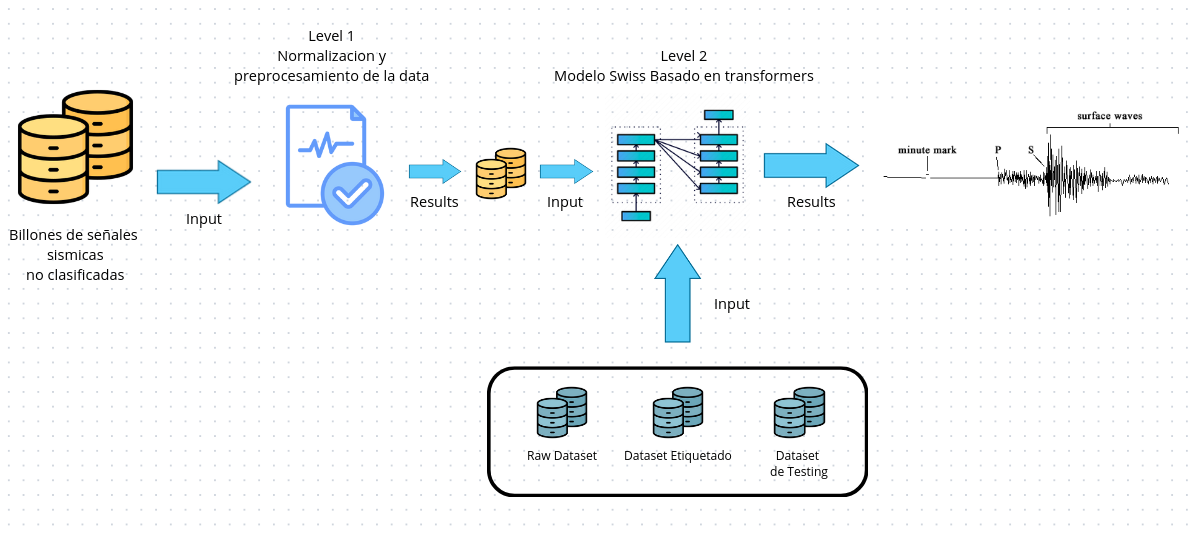
\includegraphics[scale=0.4]{figures/PIPELINE.png}
\caption{Pipeline del modelo propuesto.}
\label{Fig:Pipeline}
\end{center}
\end{figure*}

\section{Estructura de la tesis}

La presente tesis se encuentra organizada en cinco capítulos, los cuales se detallan a continuación:

\begin{itemize}
    \item \textbf{Capítulo 1 – Introducción}: Se presenta el contexto general del problema, así como la importancia de la detección temprana de ondas sísmicas. Se describe el objetivo principal del trabajo, la motivación detrás del uso de modelos basados en \textit{deep learning}, especialmente \textit{transformers}, y las contribuciones específicas de la investigación. Finalmente, se detalla la organización general del documento.

    \item \textbf{Capítulo 2 – Estado del Arte}: Se realiza una revisión de los métodos existentes para la detección de fases sísmicas, tanto tradicionales como basados en técnicas de inteligencia artificial. Se discuten modelos relevantes como \textit{EQTransformer}, \textit{PhaseNet}, y otras arquitecturas de redes neuronales profundas, así como sus fortalezas, limitaciones y oportunidades de mejora.

    \item \textbf{Capítulo 3 – Metodología}: Se describe detalladamente el enfoque propuesto, incluyendo la arquitectura del modelo \textit{transformer}, las técnicas de preprocesamiento aplicadas a las señales sísmicas, y la configuración del proceso de entrenamiento. Además, se presenta el conjunto de datos utilizado, las métricas de evaluación y el \textit{pipeline} completo del sistema.

    \item \textbf{Capítulo 4 – Resultados y análisis}: Se presentan los resultados obtenidos por el modelo propuesto en distintas métricas de desempeño. Se comparan estos resultados con enfoques tradicionales y modelos existentes. También se analiza la interpretabilidad del modelo y su capacidad para generalizar a nuevos datos.

    \item \textbf{Capítulo 5 – Conclusiones y trabajos futuros}: Se resumen las principales conclusiones de la investigación, destacando los logros alcanzados y las limitaciones identificadas. Finalmente, se proponen líneas futuras de trabajo orientadas a mejorar el rendimiento del modelo, adaptarlo a otras regiones geográficas, y explorar nuevas aplicaciones dentro del ámbito de la sismología computacional.
\end{itemize}
